\documentclass[xcolor={dvipsnames},pdf, hyperref={colorlinks=true, citecolor=ForestGreen, linkcolor=BlueViolet, urlcolor=Magenta}]{beamer}
\usetheme{Frankfurt}  
\usecolortheme{whale}
\usepackage{tikz} 
\usepackage{graphicx}
\usepackage{dsfont}
\usepackage{hyperref}
\usepackage{alltt}
\usepackage{enumerate}
\usepackage{amsthm}
\theoremstyle{definition}
\newtheorem{exmp}{Example}[section]
\usepackage{verbatim}               % useful for \begin{comment} and \end{comment}
\usepackage{eurosym}                % used for euro symbol
\usepackage{caption} 
\usepackage{graphicx}
\usepackage{adjustbox}
\graphicspath{{Figures/}}
\usepackage{subcaption}
\usepackage{color}
\usepackage{float}
\usepackage{amssymb}
\usepackage{sgamevar}
\usepackage{remreset}% tiny package containing just the \@removefromreset command
\makeatletter
\@removefromreset{subsection}{section}
\makeatother
\setcounter{subsection}{1}



\newcommand{\defn}[1]{\textbf{#1}}


%Instructor version
\newcommand{\blank}[0]{}
\newcommand{\ddp}[1]{{\textcolor{ForestGreen}{#1}}} 
\newcommand{\dd}[1]{{\underline{\textcolor{ForestGreen}{#1}}}}

%Student version
%\newcommand{\blank}[0]{\vspace{2em}}
%\newcommand{\dd}[1]{\underline{\hspace{3cm}}} 
%\newcommand{\ddp}[1]{}

\addtobeamertemplate{navigation symbols}{}{%
	\usebeamerfont{footline}%
	\usebeamercolor[fg]{footline}%
	\hspace{1em}%
	\insertframenumber/\inserttotalframenumber
}

\section{Classical Theory}

%% preamble
\title{Money Growth and Inflation}
\author{David A. D\'iaz}
\institute{UNC Chapel Hill}
\date{}

\AtBeginSection[] %Section links on slides

\begin{document} 
	
	\begin{frame}
		
		\titlepage
		
	\end{frame}

\begin{frame}{Money Growth and Inflation}
\begin{itemize}
	\item \textbf{Principle 9: Prices Rise when the Government Prints Too Much Money}
	\item We have already discussed how to calculate inflation using the \dd{CPI} or \dd{GDP deflator}. 
	\item Moreover, we have discussed how inflation can decrease purchasing power over time.
	\item This section examines a theory that explains why an economy experiences inflation and how much. We also consider some other costs of inflation.
\end{itemize}
\end{frame}

\begin{frame}{Classical Theory of Inflation}
\begin{itemize}
	\item The economy's overall price level can be viewed two ways:
	
	\begin{enumerate}
		\item The price of a basket of goods and services.
		\item A measure of the value of money.
	\end{enumerate}
	
	\item Let $P$ represent the price level. $P$ measures the number of dollars needed to buy a basket of goods and services.
	\item So, how many goods and services could be bought with \$1? \dd{$1/P$}.
	\item $1/P$ is the \dd{value} of money measured in terms of goods and services.
	\item Thus, when the price level rises, the value of money \dd{falls}.
\end{itemize}
\end{frame}

\begin{frame}{Classical Theory of Inflation}
	\begin{itemize}
		\item Just like other markets, the value of money is determined by supply and demand.
		\item For the sake of simplicity, we will assume that the quantity of money supplied is controlled perfectly by the Fed, implying that the money supply curve is \dd{perfectly inelastic}.
	
	\end{itemize}
\end{frame}

\begin{frame}{Classical Theory of Inflation}
\begin{itemize}

	\item The demand for money is determined by a few factors:
	\begin{enumerate}
		\item How much wealth people wish to hold in liquid form
		\item Access to credit
		\item Interest rates of less liquid stores of value
		\item The average level of prices 
	\end{enumerate}

\end{itemize}
\end{frame}

\begin{frame}{Classical Theory of Inflation}
	\begin{itemize}
		\item Remember that the main function of money is that it is used as a \dd{medium of exchange}. Thus, the higher prices are, the more money a typical transaction requires, and so the quantity of money demanded will \dd{increase} as the price level increases.
		\item Equivalently, we can say that the quantity of money demanded increases as the value of money \dd{decreases}.
	
	\end{itemize}
\end{frame}

\begin{frame}{Classical Theory of Inflation}
\begin{itemize}
	\item Balancing the quantity of money supplied and demanded depends on the time horizon being considered. For the purposes of this section, we will only examine the long run. 
	\item In the long run, money supply and money demand are brought into equilibrium by the \dd{overall price level}.
\end{itemize}
\end{frame}


\begin{frame}{Classical Theory of Inflation}
	\begin{itemize}
		\item 	Suppose the Fed takes some action that increases the supply of money. 
		
		\begin{figure}[H]
			\centering
			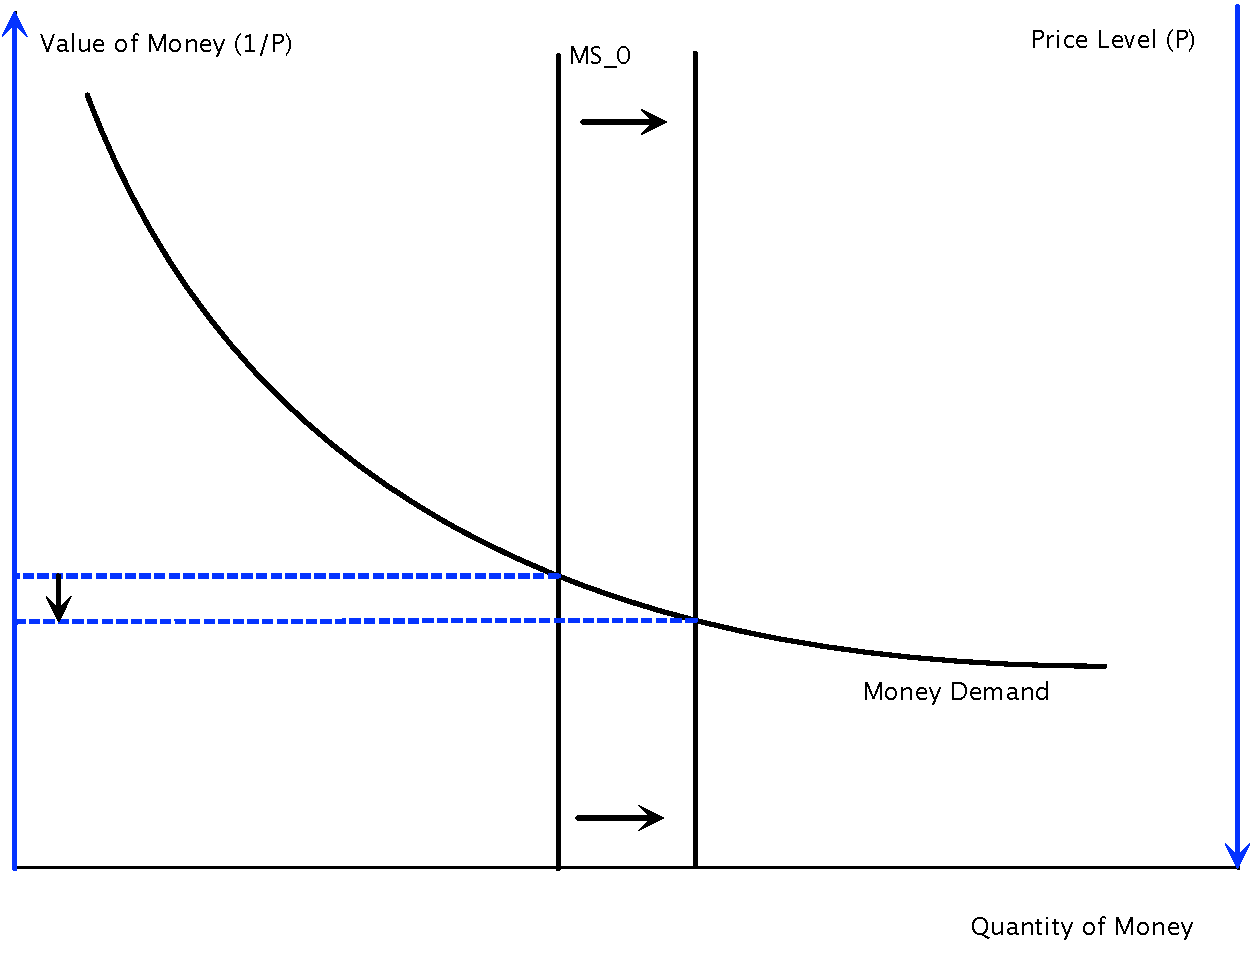
\includegraphics[scale=.3]{plot94.pdf}
			\caption{Monetary Injection}
		\end{figure}
	
	\end{itemize}
\end{frame}



\begin{frame}{The Quantity Theory}
	\begin{itemize}
	\item \defn{Quantity Theory of Money:} A theory asserting that the quantity of money available determines the price level and that changes in the money supply determine the inflation rate.
		\item Division of economic variables:
		\begin{enumerate}
			\item \textbf{Nominal variables:} Variables measured in monetary units without accounting for the effects of inflation.
			\item \textbf{Real variables:} Variables measured in physical units or in terms of purchasing power (i.e., taking inflation into account).
		\end{enumerate}
		
		\item This separation is referred to as the \dd{classical dichotomy}. 
		\item Examples of real variables:
		\begin{enumerate}
			\item Real wages
			\item Real interest rates
			\item Relative prices
		\end{enumerate}
	\end{itemize}
\end{frame}

\begin{frame}{Classical Theory of Inflation}
	\begin{itemize}
		\item According to this analysis, \dd{nominal variables} are influenced by changes in the monetary system, while \dd{real variables} are by and large not affected by money.
		\item This second point is referred to as \dd{monetary neutrality}.
		\item This is true in the long run, but not necessarily in the short run. We will examine the short-run effects of monetary changes later. Money is \dd{``neutral''} in the long run because it has no effect on real variables.
	\end{itemize}
\end{frame}

\begin{frame}{The Quantity Equation}
	\begin{itemize}
		\item \defn{Money velocity ($v$):} The rate at which money changes hands.
		\item \defn{The Quantity equation:} \[M \times v = P \times Y\]
		\item We can express this equation in percent change terms as \[\vec{M} + \vec{v} = \pi + \vec{Y}\]
	
	\end{itemize}
\end{frame}

\begin{frame}{The Quantity Equation}
\begin{itemize}
	\item Because the velocity of money is relatively stable over time, it is generally safe to assume that $\vec{v} = $ \dd{0}. Thus, a change in $M$ leads to a proportional change in $P \times Y$. 
	\item Because money is neutral, it does not affect output and so the entire change in $M$ is reflected in the changes in the \dd{price level} in the long run. 
\end{itemize}
\end{frame}


\begin{frame}{The Quantity Equation}
\begin{exmp}
	It is sometimes suggested that the Fed try to achieve zero inflation. If velocity is constant, what does the rate of money growth have to be in order to achieve this outcome? What if the Fed wanted inflation to be 3\%?
\end{exmp} 
\ddp{\pause $\vec{M} + \vec{v} = \pi^* + \vec{Y}$, where $\vec{v} = 0$ and $\pi^* = 0 \Rightarrow \vec{M} = \vec{Y}$. \\
	\pause If $\pi^* = 3$, then $\vec{M} = \vec{Y} + 3\%$.}
\end{frame}

\section{Inflation and Interest}

\begin{frame}{The Fisher Effect}
\begin{itemize}
	\item \textbf{Nominal interest rate}: The advertised rate of return that does not take into account \dd{inflation}. 
	\item \textbf{Real interest rate}: Corrects the nominal rate for inflation and tells you how your purchasing power changes over time.
	\item The relationship between the variables is \dd{$r = i - \pi$}.
	\item The equilibrium real interest rate is determined by the market for loanable funds and the growth of the money supply determines the inflation rate. 
\end{itemize}
\end{frame}

\begin{frame}{The Fisher Effect}
	\begin{itemize}
		\item \defn{Fisher Effect:} The one-for-one adjustment of the nominal interest rate to the inflation rate.
		\item Because loans are set before inflation occurs, a lender that wishes the make a certain real rate of return must anticipate what inflation will be. This is called the \dd{expected} inflation. 
		\item Nominal interest rates are set using the equation \dd{$i = r^* + \pi^e$}.
		\item In the long run, it will be the case that the nominal interest rate adjusts to expected inflation, and expected inflation moves with actual inflation.
	\end{itemize}
\end{frame}

\begin{frame}{The Costs of Inflation}
	\begin{itemize}
		\item The Inflation Fallacy: Inflation in incomes goes hand-in-hand with inflation of prices. So, inflation itself does not lead to decreases in purchasing power. It is relative to the increase in wages. What matters to individuals are whether or not real wages are increasing or decreasing.
		\item Shoeleather costs: The resources wasted when inflation encourages people to reduce their money holdings. They might make more frequent trips to purchase goods, etc. and this time and effort wasted on unneeded trips is inefficient.
		\item Menu costs: The costs of changing prices. Both this and shoeleather costs are more of a factor in cases of hyperinflation.
	\end{itemize}
\end{frame}

\begin{frame}{The Costs of Inflation}
	\begin{itemize}
	\item Relative-Price Variability: Because prices only change occasionally, inflation causes relative prices to vary more than they otherwise would. Distorted relative prices leads to distorted consumer decisions and thus misallocation of resources.
		\item Tax Distortions: Inflation discourages savings in the context of taxes on capital gains or interest income. Inflation  exaggerates these gains and increases the tax burden on this type of income.
	\item Deflation: Many of the same costs as inflation, but usually deflation also indicates deeper economic issues.
	\end{itemize}
\end{frame}

\begin{frame}{The Costs of Inflation}
	\begin{itemize}
	\item Redistribution of Wealth: Rising inflation diminishes the real value of debts 
	\begin{itemize}
	\item Lenders set nominal interest rates as $i = r^* + \pi^e$
	\item Actual rate of return is given by $r_{actual} = i\ - \pi$ 
	\item We can rewrite this as $r_{actual} = r^* + (\pi^e - \pi)$
	\end{itemize}
	\item Thus, if inflation is greater than expected the real return is less than the expected return on the loan and wealth is transferred from lenders to borrowers. \item If inflation is less than expected, then wealth is transferred from borrowers to lenders.
	\end{itemize}
\end{frame}


\begin{frame}{The Costs of Inflation}
\begin{exmp}
	\scriptsize
	Consider the table below. In each case, state which party was hurt more: the bank, the mortgage holder, or neither. 
	
	\begin{table}[ht]
		\centering
		\begin{tabular}{ c|c |c}        
			
			Expected Inflation ($\pi^e$) & Actual Inflation ($\pi$) & Hurt?\\
			\hline
			4\% & 10\% & \pause \ddp{Banks: $\pi > \pi^e$} \\
			10\% & 4\% & \pause \ddp{Mortgage holders: $\pi < \pi^e$} \\
			-3\% & 0\% & \pause \ddp{Banks: $\pi > \pi^e$} \\
			-3\% & -6\%  & \pause \ddp{Mortgage holders: $\pi < \pi^e$}\\
		\end{tabular}
	\end{table} 
\end{exmp}
\end{frame}

\begin{frame}{Readings and Assignments}
\begin{itemize}
	\item Today: Mankiw Ch. 30
	\item Next time: Mankiw Ch. 32
	\item Problem Set 6, section 2
\end{itemize}
\end{frame}

\end{document}